% This file was created by matplotlib2tikz v0.7.4.
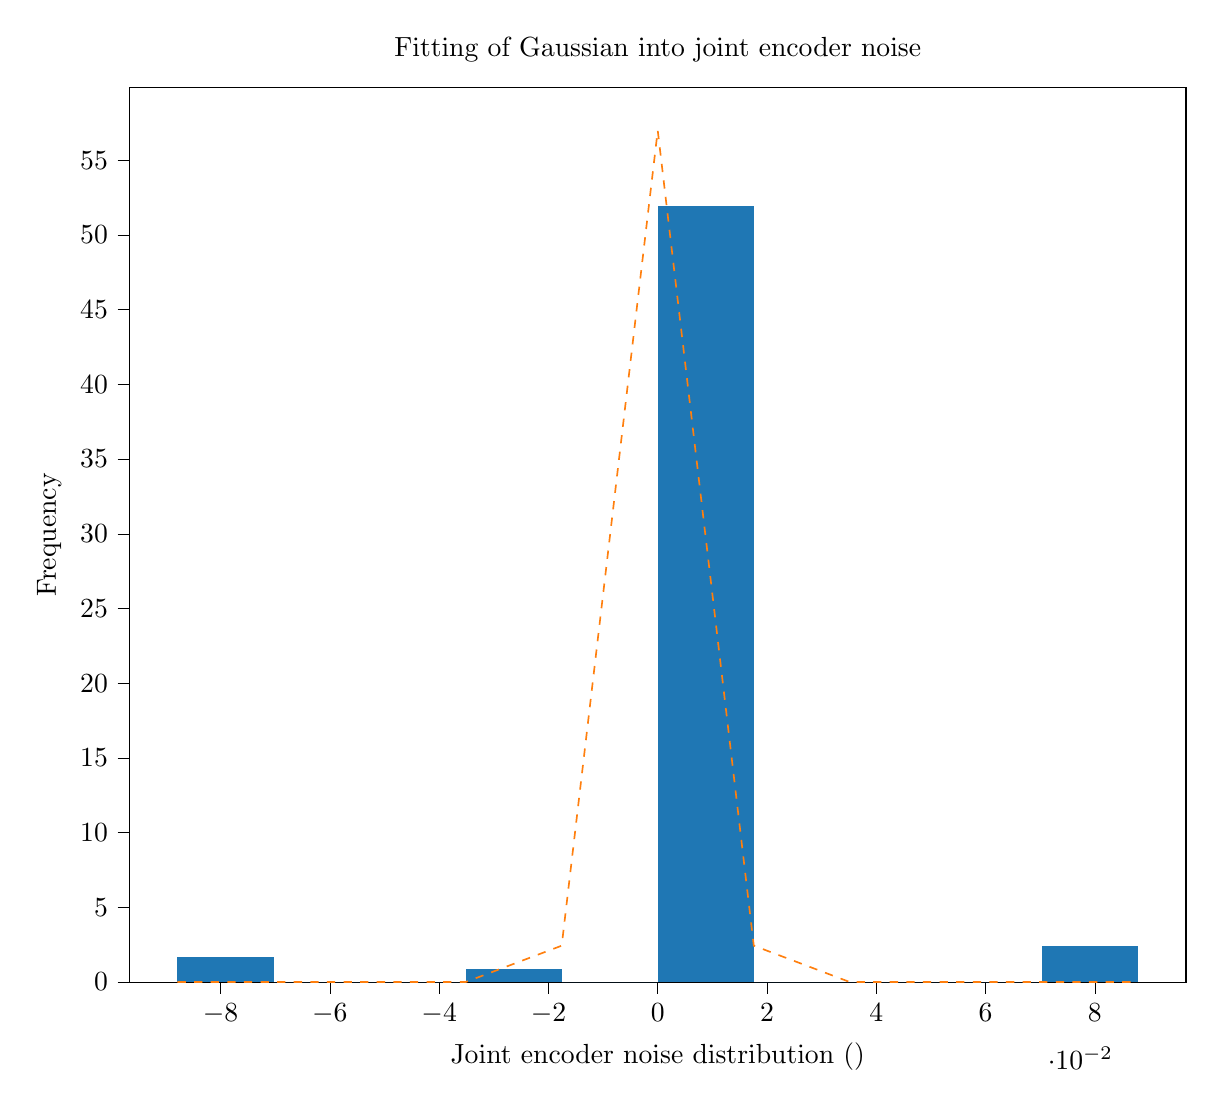
\begin{tikzpicture}

\definecolor{color0}{rgb}{0.12156862745098,0.466666666666667,0.705882352941177}
\definecolor{color1}{rgb}{1,0.498039215686275,0.0549019607843137}

\begin{axis}[
tick align=outside,
tick pos=left,
title={Fitting of Gaussian into joint encoder noise},
width=15cm,
x grid style={white!69.01960784313725!black},
xlabel={Joint encoder noise distribution (\(\displaystyle \degree\))},
xmin=-0.0966799616637501, xmax=0.0966799616637024,
xtick style={color=black},
y grid style={white!69.01960784313725!black},
ylabel={Frequency},
ymin=0, ymax=59.8413420602149,
ytick style={color=black}
]
\draw[fill=color0,draw opacity=0] (axis cs:-0.087890874239775,0) rectangle (axis cs:-0.0703126993918247,1.68171830791555);
\draw[fill=color0,draw opacity=0] (axis cs:-0.0703126993918247,0) rectangle (axis cs:-0.0527345245438745,0);
\draw[fill=color0,draw opacity=0] (axis cs:-0.0527345245438745,0) rectangle (axis cs:-0.0351563496959243,0);
\draw[fill=color0,draw opacity=0] (axis cs:-0.0351563496959243,0) rectangle (axis cs:-0.0175781748479741,0.855956547042105);
\draw[fill=color0,draw opacity=0] (axis cs:-0.0175781748479741,0) rectangle (axis cs:-2.38559172416331e-14,0);
\draw[fill=color0,draw opacity=0] (axis cs:-2.38559172416331e-14,0) rectangle (axis cs:0.0175781748479264,51.9057126351254);
\draw[fill=color0,draw opacity=0] (axis cs:0.0175781748479264,0) rectangle (axis cs:0.0351563496958766,0);
\draw[fill=color0,draw opacity=0] (axis cs:0.0351563496958766,0) rectangle (axis cs:0.0527345245438268,0);
\draw[fill=color0,draw opacity=0] (axis cs:0.0527345245438268,0) rectangle (axis cs:0.070312699391777,0);
\draw[fill=color0,draw opacity=0] (axis cs:0.070312699391777,0) rectangle (axis cs:0.0878908742397273,2.44534007406507);
\addplot [semithick, color1, dashed]
table {%
-0.087890874239775 3.33231062514069e-33
-0.0703126993918247 7.02505025071183e-21
-0.0527345245438745 2.7033860508016e-11
-0.0351563496959243 0.000189898431725009
-0.0175781748479741 2.43494616603573
-2.38559172416331e-14 56.9917543430618
0.0175781748479264 2.43494616607742
0.0351563496958766 0.000189898431731511
0.0527345245438268 2.70338605094043e-11
0.070312699391777 7.02505025119292e-21
0.0878908742397273 3.33231062542587e-33
};
\end{axis}

\end{tikzpicture}